\chapter{Conclusion générale}
%\colorbox{yellow}{refondre}
%\section{Conclusion État de l'art}

%soutenabilité
Dans notre traitement de la notion de soutenabilité, nous avons vu la multiplicité du concept et en avons fait une synthèse.
Nous comprenons maintenant que la soutenabilité n'existe que par l'action évaluative de sujets.
En observant la méthodologie actuelle de l'ACV, nous avons vu qu'elle n'était pas en mesure \emph{de juger si une activité de transformation produisait consensus et institutionnalisation dans le cadre de l'évolution de cultures humaines, sans fin discernable et involontaire de leurs faits, par l'action ou l'inaction, pour lesdits sujets, ou pour l'écosystème, dans sa diversité, sa complexité et sa capacité à supporter la vie.}
\textbf{En somme l'\gls{ACV} ne permettait pas de traiter de soutenabilité.}

\begin{figure}[htbp]
\centering
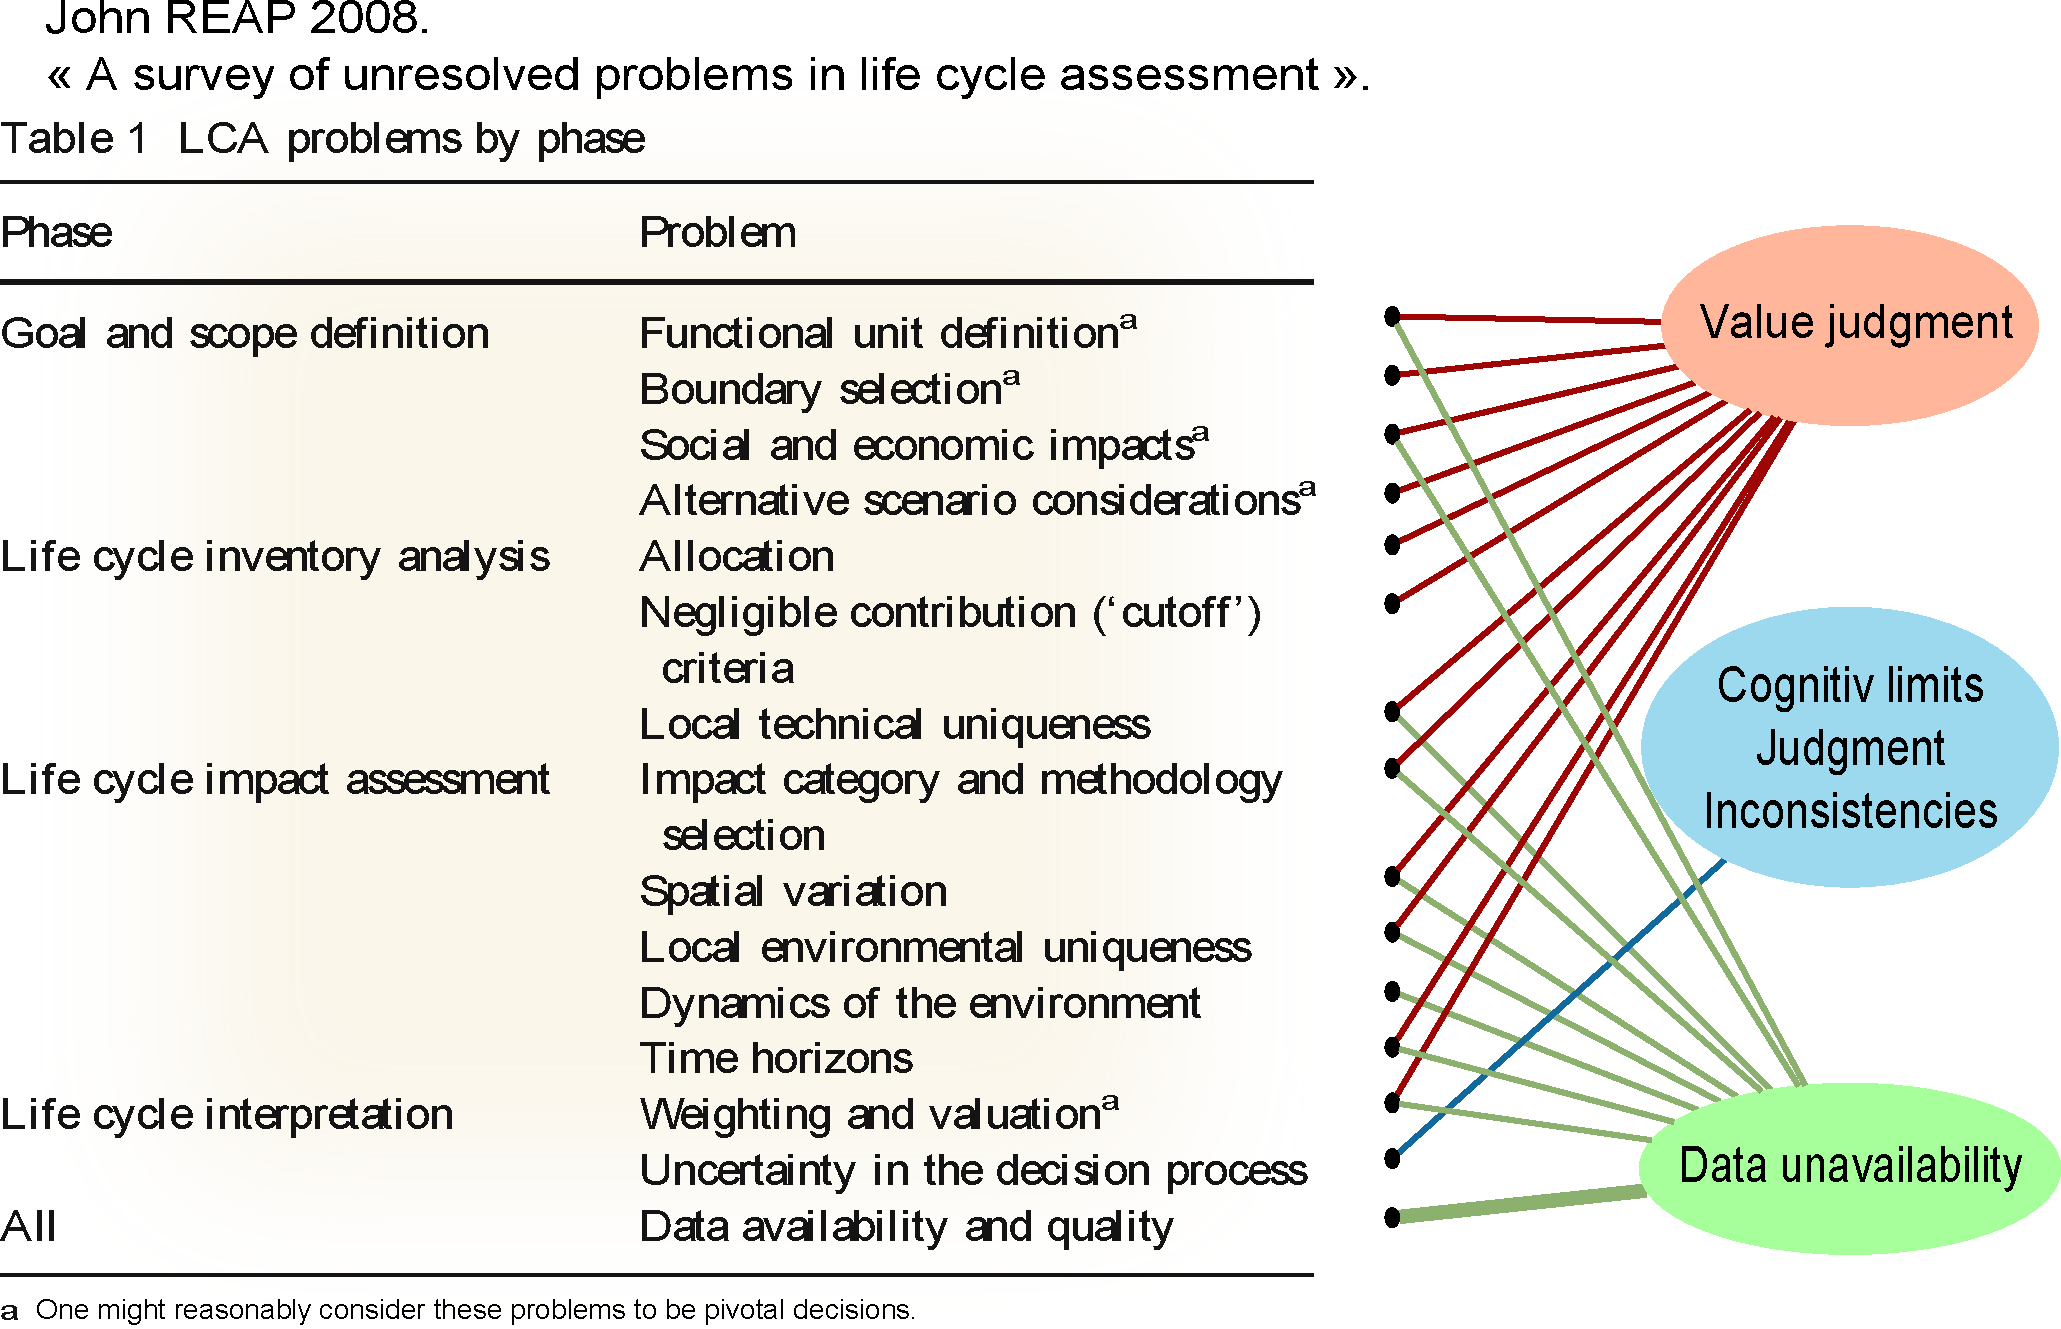
\includegraphics[width=\textwidth]{/home/rudy/Documents/rudy/01_These/11_production/01_COMMUNICATION/figures/what_we_missed_untill_now.pdf}
\caption{Synthèse des axes de résolutions.}
\label{fig:what_we_missed_untill_now}
\end{figure}

%reconception
Mais nous avons ensuite entrepris de \textbf{la concevoir à nouveau}, suivant les axes de résolution de la figure~\ref{fig:what_we_missed_untill_now}, \emph{pour permettre de façon opérationnelle l'évaluation de la soutenabilité}.

Nous sommes convaincu qu'il ne peut y avoir uniformisation totale de la soutenabilité, et à ce sens il ne peut y avoir \textit{un} indicateur de soutenabilité.
Il ne s'agit pas d'une caractéristique d'un état mais, comme la définition le souligne, plutôt d'un processus.
La soutenabilité n'a pas d’existence naturelle, c'est un concept, un artefact, le fruit d'une évaluation.
Elle peut toutefois être \emph{un} objectif utopique pour des individus comme des groupes et être poursuivie de façon \emph{rationnelle} et produire une forme volontaire d'unité de l'humanité au travers la mutualisation de nos ressources pour l'obtention de valeurs (consistantes), communes.
En quelque sorte, elle peut être un objectif auto-réalisé par sa poursuite.

%decision multicritère et jugement de valeurs
\textbf{L'ACV pourra répondre aux questions de soutenabilité.}
Mais les aménagements sont nombreux et la désignation peut-être inadéquate.
Le modèle conceptuel que nous avançons permet d'ailleurs de traiter la question selon les six concepts présents dans la littérature (\ref{6concepts_soutenabilité}), suivant que le modèle de jugement introduit répond à ces définitions.
Grâce à une première phase d'existence, la pensée en cycle de vie a jeté des fondations sur la criticité de la multidimensionnalité, l'analyse systémique, le processus itératif et le caractère décisionnel.
Cet état d'avancement, il faut effectivement en premier lieu le reconnaître et le faire reconnaître~\cite[conclusion p.244]{klopffer_background_2014}.
\textit{Mais il convient maintenant surtout de le dépasser~!}
Il reste à l'ACV à acter de sa pluridisciplinarité, voir transdisciplinarité, qui la caractérise.
Une fois cela acquis, il conviendra d'organiser la réception et le traitement des jugements moraux des décideurs.
Cette lourde tâche, qui nécessitera l'expertise de linguistes, psychologues et de mathématiciens, associé aux porteurs des jugements de valeurs eux-même, afin d'établir les échelles adéquates et le modèle interrogatoire, n'est pas cantonnée à la question de la soutenabilité.
\emph{Ceci est valide pour toute méthode de prise de décision qui se réclame de la rationalité.}
Car \textbf{toute décision réelle est multicritère}.
Et comme des attributs \emph{incommensurables} sont en jeu, \emph{nous ne pouvons pas nous passer de l'expression d'opinions}.
C'est sur la base du système de valeur du décideur qu'est réalisée l'évaluation, c'est donc le système évaluateur, indépendamment de l'analyste.
Pour la soutenabilité cependant, s'ajoute le concours indispensable de la société civile dans sa globalité.

%multifonctionnalité
La question de la multifonctionnalité, était jusqu'ici considérée comme non-résolue.
Plus qu'une formulation ambiguë des questions d'allocation~\cite{weidema_has_2014},
les limitations de l'ISO~14040 et de l'ILCD réside dans l'absence d'un élément central~: \emph{l'intégration globale, consistante et explicite, du jugement moral des parties-prenantes}.
Une fois (i) reconnue comme systématique à tout procédé et (ii) abordée sous l'angle de la multi-dimensionnalité, la problématique est résolue de façon courante via les \gls{ADMC} de la décennie 70.

% reformer des normes iso ilcd et canons de la décision multicritère
Le traitement de ce problème global étant maintenant claire il faut qu'il intègre le cadre normalisé de la discipline.
L'étape additionnelle de \emph{déclaration de valeurs}, pour des raisons de consistance, devrait viser l'ensemble de la multi-dimensionnalité, c-a-d (selon les termes actuels) à la fois les attributs des flux pour le traitement de la multifonctionnalité \textbf{et} les \emph{impacts} pour l'interprétation finale.
Les conséquences du modèles présentés par partition sur la question du traitement des déchets, mettent à jour d'ailleurs fort clairement l'\textbf{unicité du domaine des fonctions et des impacts.}
Cette étape de déclaration d'opinion devrait être traitée avant même la définition du but de l'étude~\cite{patard_life_2015}.
Elle serait une étape indépendante de l'ACV, bien que fournissant une part d'information cruciale à sa réalisation.
Elle pourrait d'ailleurs servir d'autres méthodologies d'\gls{ADMC}, bien que nous ne voyons pas dans quelle mesure il serait raisonné de tronquer l'espace temporel et spatial, i.e. de ne pas suivre la globalité du cycle de vie.

%traitement de l'opinion et nécessité
Ce 'découpage', observation - opinions, permettra un processus de revue effectif des ACV.
%L'application effective du jugement du décideur pourrait être contrôlée.
Les bases de données contiendrait alors les descriptions des systèmes techniques, environnementaux et sociaux.
\textbf{Il sera donc possible, par son application, de fournir la dissociation de l'observation et de la modélisation.}
Cette dissociation entre faits et opinions ainsi que le rattachement d'opinions aux preneurs de décisions nécessitent des précautions particulières entre anonymisation, pseudonymat et déclarations nominatives.
Le factuel est entré nominativement pour des questions de  vérification et responsabilité.
L'opinion devrait \textit{pouvoir} être gardée confidentielle\footnote{Réalisable à l’échelle individuelle, mais pas en groupe.}.
\textbf{Mais pour les décisions en groupe distribué, nécessaire à la soutenabilité, les caractéristiques du modèle actuel du vote démocratique~: transparence, confidentialité, anonymat, unicité, sincérité, ne peuvent être validées.}
Une gouvernance globale et soutenable ne semble pas applicable sans se séparer de la confidentialité et de l'anonymat.
Mais ceci reste problématique du fait que la sincérité peut être brisé par coercition sur des déclarants nominatifs.
Ce modèle n'est donc réalisable qu'en l'instauration d'autres mécanismes~: (i) tirage au sort pour l'appareil de gouvernance et dans chaque pouvoir (ii) salaire universelle, (iii) co-propriété d'usage des moyens de production.
Il reste que jusqu'ici la transparence indirecte des processus électroniques fait obstacle à la confiance.
Le niveau d'éducation des populations pour une société à ce stade de sophistication doit s’accroître\footnote{Rappelons que nous faisons appel à des techniques d'\gls{ADMC}, qui si elles peuvent être vulgarisées, nécessite des concepts complexes.}.

%économie politique
Le traitement de la multi-fonctionnalité a fait ressortir les discours sur les valeurs d'usages et les valeurs d'échanges qui sont nettement plus fréquent chez les économistes.
La résolution peut être faite soit par \emph{partition}, soit par \emph{expansion}, sans qu'il soit \textbf{nullement nécessaire d'introduire de \emph{substituabilité}}.
Puisque l'équipe de \citeauthor{majeau-bettez_unified_2014}, a produit son formalisme tant pour l'ACV que les études économiques d'input-output, il n'y a aucune raison que notre modèle ne s'y applique également.
Notre travail, relevant les idéologies dominantes et leur imbrication à l'outil d'évaluation, souligne combien il n'y a d'économie, que d'\emph{\textbf{économie politique}}, au sens de sa critique marxienne.

%rationalité et inconsistance
Les inconsistances d'opinions ne doivent pas donner lieu à une tentative de leurs réductions \emph{à dimensions constantes de la matrice de jugements.}
Elles doivent être l'occasion de l'extension dimensionnelle de celle-ci.
La confrontation de systèmes de valeur issues de groupes hétérogènes sur leur inconsistance globale est elle-même le processus de production du consensus et d'institutionnalisation~:
(i) Par la recherche d'un système consistent depuis des groupes en contradiction il génère la recherche du consensus, c-a-d la recherche des valeurs communes primordiales.
(ii) Le processus génère les organes qui défendront ces valeurs ou les reconnaîtrons comme normatives~: institutionnalisation.

%dissémination scientifique
Bien évidement la résolution de la thématique de la multi-dimensionnalité appelle d'autant plus qu'il fait la synthèse des autres problèmes non-résolus, le besoin en données (déjà conséquent avant même de traiter les opinions).
La résolution de ce second thème majeur passe, outre l'emploi des technologies du web sémantique pour le gigantisme de la masse de donnée, par la refonte du système de l'enseignement supérieur et de la recherche, notamment l'appareil de publication de l'information scientifique et technique.
Pour avancer sur cette voie nous avons produit un protocole de publication où le seul point de striction restant réside dans l'hébergement.
Ce à quoi nous ajoutons que la solution probable à ce dernier point est une forme de réseau de communication distribuée, hors des infrastructures de communication dominées par des organes bourgeois à but lucratif.
C'est à dire un réseau de communication complet en co-propriété d'usage.
L'appareil de gouvernance de l'outil (rôles d'administrateurs), doivent donc également comporter du tirage au sort.
Repensé, notre système de dissémination de la recherche publique est fondu dans les canons de l'open-source et du libre, c-a-d dans la transition complète à l'économie du don.
Plus exactement, il doit passer à un modèle d'acteurs scientifiques agissant dans le paradigme du don et soutenu par l'universalisation du salaire et du support à la recherche par subvention démocratiquement allouée.
C'est une conséquence directe, dans la Recherche, du passage au modèle de publication de Journaux Scientifiques Libres, de la capacité de libération des contraintes verticales et de l'ouverture à la société civile.

%\input{concl_metalo}

\keybox{
Les solutions organisationnelles recèlent, selon nos travaux, plus de potentiel que les solutions technologiques.

La capacité de l'\emph{ACV re-conçue} à se développer en tant que science, sera directement liée à notre capacité à dissocier, observation, opinion et leur traitement conjoint.
Les façons dont nous organiserons la détermination des jugements de valeur pour nos processus de décisions collectifs seront les miroirs de nos cultures.
}

